\documentclass[11pt,a4paper]{scrartcl}

% ********************************************************************    
% Packages
% ********************************************************************
\usepackage[utf8]{inputenc}
\usepackage{tikz}
\usetikzlibrary{shadings}
\usepackage[outline]{contour}
\usepackage{pgfplots}
% \usepackage{tikz-3dplot}
\usepackage{graphicx}
\usepackage{algorithm}% http://ctan.org/pkg/algorithms
\usepackage{algpseudocode}% http://ctan.org/pkg/algorithmicx
\usepackage{subfig}
\usepackage{amsmath,amssymb}
\usepackage{mathtools}
\usepackage{braket}
\usepackage{hyperref}
\usepackage{slashed}
\usepackage{pifont}
\usepackage{tcolorbox}
\usepackage{qcircuit}
\usepackage{amsthm}
\usepackage{amsfonts}
\usepackage{lmodern}
\usepackage{dsfont}
\usepackage{times}
\usepackage{bbm}
\usepackage{wrapfig}
\usepackage[T1]{fontenc}

\usepackage[backend=bibtex,citestyle=authoryear,isbn=false,url=false,doi=false]{biblatex}
\addbibresource{Bibliography.bib}

\DeclareMathOperator{\Tr}{Tr}
\newcommand{\R}{\mathbb{R}}
\newcommand{\N}{\mathbb{N}}
\newcommand{\C}{\mathbb{C}}
\newcommand{\Z}{\mathbb{Z}}

\newtheorem{lemm}{Lemma}

% ********************************************************************    
% Settings
% ********************************************************************

% biblatex
\DeclareCiteCommand{\myfootcite}
  {\footnotetext{\usebibmacro{prenote}}
  {\usebibmacro{citeindex}%
    \usebibmacro{author}
    \printfield{journaltitle}
    \printfield{volume}
    (\printfield{year})}
  {\multicitedelim}
  {\usebibmacro{postnote}}}



%TODO Name does not appear, layout
% meta
\author{Daniel Brosch}
\title{Quantum SDP-solver}
\date{
  Convex Optimization Seminar \\
  Bad Honnef \\
  August 7 -- 9, 2017
}

\begin{document}
\maketitle
{
\centering
\Large
\vspace{4cm}
Mathematisches Institut\\
Mathematisch-Naturwissenschaftliche Fakultät\\
Universität zu Köln\\
}

\thispagestyle{empty}
\newpage
\pagenumbering{roman}
\tableofcontents
\thispagestyle{empty}
\newpage
\pagestyle{headings}
\pagenumbering{arabic}

\section{Introduction}
\subsection{Quantum computing}
%TODO
TODO
\subsection{Semidefinite programming}
Semidefinite programming can be used to solve a wide range of problems, some examples include solving graph problems (e.g. approximating MAXCUT), machine learning (e.g. face recognition) and general polynomial optimization. This means that faster SDP-solvers would have potential uses in many different fields, and a fast quantum-SDP-solver could open ways to multiple new applications for quantum computers.
The general form of semidefinite programs is:
\begin{align*}
\text{Primal form:}\quad && \text{Dual form:}\quad &\\
\max\quad &\Tr(CX) &\min\quad &b^T y\\
\text{s.t.}\quad &\Tr(A_jX)\leq b_j \text{ for }1\leq j\leq m &\text{s.t.}\quad &\sum_{j=1}^m y_j A_j-C\succeq 0\\
& x\succeq 0 && y\geq 0
\end{align*}
%TODO which norm is this exactly?
Where $A_1,\ldots, A_m, C$ are hermitian matrices. During this work we will assume that $\|A_j\|\leq 1$ and $\|C\|\leq 1$, which is not a restriction, because we can scale $A$, $C$ and $b$ equally without changing the problem (We just have to remember to scale the maximum/minimum back at the end). But we will further assume that we know positive constants $R$ and $r$, so that there is an optimal solution of the primal problem with $\Tr X\leq R$ ($A_1=\mathbbm{1}$, $b_1=R$) and similarily an optimal solution of the dual problem with $\|y\|_1\leq r$. 

\subsection{Arora-Kale SDP solver}
%TODO
The quantum algorithm, which is this paper about, is based on a classical algorithm developed by Arora and Kale. It is an SDP-solver in the form of a matrix multiplicative weight algorithm. While I wont go into details of its workings here (for that I refer to Markus' part of the presentation or (TODO arora kale source)), we need to understand some parts: The basic idea of the algorithm is to start with a positive semidefinite canditate solution $X^{(1)}$ (which does not have to be a feasible solution), then use it with a subroutine called Oracle to find a candidate  dual solution (again not necessarily feasible) $y^{(1)}$, with $b^Ty\leq\alpha$. The value $\alpha$ is here a guess for the optimal value of the SDP, for which we can search binary by repeating the algorithm. With this $y$ we can then find a better candidate for the primal solution and repeat this whole process. It can be shown that after enough repetitions the average of all the $y^{(i)}$ is close to dual feasible, and can be tweaked to get a dual feasible solution with $b^Ty\leq\alpha$.

The quantum speed-ups both have to do with the Oracle, so we will take a closer look at it here. Its task is to find a candidate dual solution $y$ from the polytope

\begin{align*}
\mathcal{P}_\varepsilon (X^{(i)})=\{y\in\R^m | &b^Ty\leq\alpha,\\
 &\Tr\left(\left(\sum_{j=1}^m y_jA_j-C\right)X^{(i)}\right)\geq -\varepsilon,\\
 & y\geq 0\}
\end{align*}

The second line is a relaxation of the condition of the dual programm, that $\sum_{j=1}^m y_jA_j-C$ is positive semidefinite, instead it only requires the inner product with a specific psd matrix not to be too negative. 
Now we can see that we dont even need to know every entry of the matrices $A_j, C$ and $X^{(i)}$, instead it is enough to know the trace inner products between them:

\begin{equation*}
\Tr\left(\left(\sum_{j=1}^m y_jA_j-C\right)X^{(i)}\right)=\sum_{j=1}^m y_j \Tr(A_jX^{(i)})-\Tr(CX^{(i)})
\end{equation*}

It will be easier to work with normalized $\rho=\frac{X^{(i)}}{\Tr(X^{(i)})}$ instead of $X^{(i)}$, and it does not change this polytope if we scale $\varepsilon$ accordingly (remember: we know an upper bound $\Tr(X)\leq R$). And we can further see that additive approximations to these are enough as well: If we have $|a_j-\Tr(A_j\rho)|\leq \theta$ and $|c-\Tr(C\rho)|\leq \theta$ and include the upper bound for an optimal solution $\|y\|_1\leq r$ we can define a new polytope:

\begin{align*}
\tilde{\mathcal{P}}(a_1,\ldots, a_m,c)=\{y\in\R^m | &b^Ty\leq\alpha,\\
&\|y\|_1\leq r,\\
 &\sum_{j=1}^m y_j a_j\geq c,\\
 & y\geq 0\}
\end{align*}

Notice here that $\varepsilon$ does not appear in this formulation. This is because we can show that if we have a $y\in\mathcal{P}_0(X)$ with $\|y\|_1\leq r$, then

\begin{equation*}
0\leq \sum_{j=1}^m y_j \Tr(A_j\rho)-\Tr(C\rho) \leq \sum_{j=1}^m y_j (a_j+\theta)-(c-\theta) \leq  \sum_{j=1}^m y_j a_j-c +(r+1)\theta
\end{equation*}

which shows that $y$ is in $\tilde{\mathcal{P}}(a_1,\ldots,a_m, c'=c-(r+1)\theta)$. This means, because when there is a feasible solution, then $\mathcal{P}_0(\rho)$ is not empty, that $\tilde{\mathcal{P}}(a_1,\ldots,a_m, c')$ is not empty as well. It does work other way around as well: If we have a $y\in\tilde{\mathcal{P}}(a_1,\ldots,a_m, c')$, then is $y\in \mathcal{P}_{4Rr\theta}(X)$.

This means that we can work with $\tilde{\mathcal{P}}$ instead of $\mathcal{P}$ in the algorithm. Both of the quantum speed-ups have to do with this oracle.

% ************************************
\section{Quantum Speed-Ups}
% ************************************

The algorithm of Arora and Kale can be sped up using quantum computers at two points, the first of which is estimating $\Tr(A\rho)$ for a hermitian matrix $A$ and a density matrix $\rho = \frac{e^{-H}}{\Tr(e^{-H})}$, which is used as input for the Oracle.

The second speed-up is the implementation of the (general) oracle itself, which will be based on applications of known quantum algorithms.

\subsection{The input of the Oracle:}

For the oracle's input we have to approximate expressions of the form $\Tr(Ap)$ with $p=\frac{e^{-H}}{\Tr(e^{-H})}$, where $A$ and $H$ are hermitian matrices. This we can seperate into two calculations, $\Tr(Ae^{-H})$ and $\Tr(e^{-H})$.
We have seen before that we want an additive approximation of $\Tr(Ap)$, which can be reduced to multiplicative approximations of $\Tr\left(\frac{\mathbbm{1}+A/2}{4}e^{-H}\right)$ and $\Tr\left(\frac{1}{4}e^{-H}\right)$.
%TODO Proof

Important to note is here that we wont calculate these values in binary directly, instead it will first be the probability of a qubit being 0. Specifically this means we have to construct a quantum circuit, which corresponds to a unitary matrix $U$, in a way so that it turns a specified input register (e.g. $\ket{0\ldots 0}$) into a register with the first qubit as wanted.

Amiplitude estimation is then used to approximate this probability, during which $U$ and $U^{-1}$ are used multiple times.

\vspace{1cm}

Before explaining how to construct this circuit (or at least its general idea) for any semidefinite programm, we will take a look at the much simpler case of linear programming. These can be seen as the subclass of SDP, which only uses diagonal matrices. Here it means that the calculation of $\Tr(Ae^{-H})$ becomes significantly easier (and by that the one of $\Tr(e^{-H})=\Tr(\mathbbm{1}e^{-H})$ as well), as it is now just the sum of $a_{ii}e^{-h_{ii}}$ for $1\leq i\leq n$.

These values can now be approximated classically, and stored as binary values in a quantum register. These can then be transformed into the form we want using something similar to a quantum fourier transformation:

More precisely, we calculate binary approximations of $\beta=\arcsin(\sqrt{b})/\pi$, where $b\in [0,1]$ is the value we want as the probability of a qubit being 0. Let $b_0.b_1b_2b_3\ldots b_t$ be the binary represenation of $\beta$. Using one ancilla qubit we are now working with the register $\ket{1}\ket{\beta}=\ket{1}\ket{b_0}\ket{b_1}\ldots\ket{b_t}$. If we now apply $t$ controlled rotations to the first qubit, one for each bit of $\beta$, rotating by $\pi 2^{-j}$ towards $\ket{0}$ if $b_j=1$, we receive:
\begin{align*}
&\left(\sin\left(\sum_{b_i=1} \pi 2^{-i}\right)\ket{0}
+\cos\left(\sum_{b_i=1} \pi 2^{-i}\right)\ket{1}\right)
 \ket{\beta}\\
=&\left(\sin\left(\pi\beta\right)\ket{0}
+\cos\left(\pi\beta\right)\ket{1}\right)
 \ket{\beta}\\
=&(\sqrt{b}\ket{0}+\sqrt{1-b}\ket{1})\ket{\beta}
\end{align*}
For which the probability, that the first qubit is 0, is exactly $\|\sqrt{b}\ket{0}\|^2=b$.

%TODO
TODO The input of the Oracle: SDP. A lot of work, only the basic idea instead. Author develops a way to calculate "smooth" functions like $e^{-H}$ and $\sqrt{A}$ efficiently using quantum computers.



\subsection{The Oracle}

The Oracle is a subroutine used by the Arora-Kale algorithm, which calculates a candidate dual solution $y$ using a candidate primal solution $X$. As seen earlier it is not necessary for the oracle to know each entry of the semidefinite matrix $X$, instead it can use $a_j\approx\Tr(A_j\rho)$ for $j=1,\ldots,m$ and $c=\Tr(C\rho)-\varepsilon$. That means we have to calculate a $y\in \mathbb{R}^m$ with:

\begin{align*}
\|y\|_1&\leq r & \omit\rlap{Compared to the dual SDP}\\
b^T y&\leq \alpha&\min \quad &b^T y\\
a^T y&\geq c& \text{s.t. } &\sum_{j=1}^m y_j A_j - C\succeq 0\\
y&\geq 0 & &y\geq 0
\end{align*}

The first condition $\|y\|_1\leq r$ is no restriction, because we assumed that there is an optimal solution with this property. We are now going to simplify the problem. Substituting $y=Nq$ with $N=\|y\|_1$ and $\|q\|_1=1$ results in:

%Some ugly magic for rcases inside of align
\begin{equation*}
 \begin{split}
  b^T q&\leq \alpha/N\\
  a^T q&\geq c/N\\
  \begin{aligned}
   \|q\|_1\\
   q
  \end{aligned}
  &
  \begin{rcases*}
   =1\\
   \geq 0
  \end{rcases*} \text{convex combination coefficients}  \\
  0&<N\leq r
 \end{split}
\end{equation*}

This way we recieve a two-dimensional interpretation of the oracle: We want to find the convex combination of a point $P$ in the polytope $Q=\mathrm{conv}\{p_i=(b_i,a_i)\}$, which lies to the upper left of the point $(\alpha/N, c/N)$ for an $N\in (0,r]$. To understand the second condition we define $G_N$ as the upper-left quadrant starting at $(\alpha/N, c/N)$ and $G$ as the union of all the $G_N$ with $0<N\leq r$.

\vspace{1cm}

%TODO
TODO Understanding the area $G$. 4 cases, one of which is $G=\R^2$, the others are intersections of 2 half planes.

\vspace{1cm}

It is easy to see that if there is a solution $q$, then there is also a 2-sparse solution. So we can always assume that we can find a solution on one of the connecting lines $\overline{p_i p_j}$ of corners of the polytope:

{

\begin{wrapfigure}{r}{6cm}
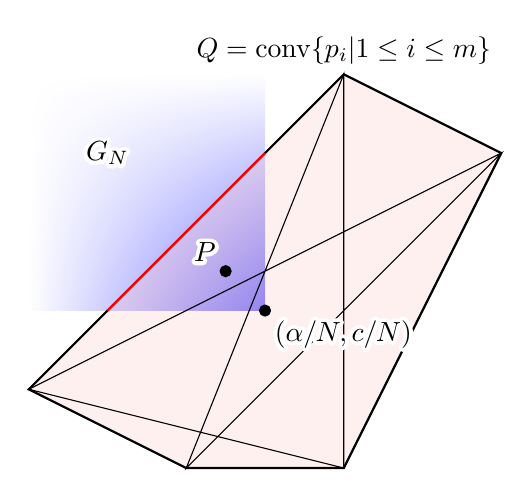
\begin{tikzpicture}
\contourlength{0.5mm};
\shade[lower right=blue!60!white] (0,0) rectangle (3,3);
\node at (1,2) {\contour{white}{$G_N$}};
\filldraw[thick, fill=red!20!white, fill opacity=0.3] (0,-1)--(4,3)--(6,2)--(4,-2)--(2,-2)--cycle;
\draw[red, thick] (1,0)--(3,2);
\node[anchor=south] at (4,3) {$Q=\mathrm{conv}\{p_i|1\leq i \leq m\}$};
\draw (0,-1)--(6,2)--(2,-2)--(4,3)--(4,-2)--cycle;
\filldraw (2.5,0.5) circle(0.07) node[anchor=south east]{\contour{white}{$P$}};
\filldraw (3,0) circle(0.07) node[anchor=north west]{\contour{white}{$(\alpha/N,c/N)$}};
\end{tikzpicture}
\end{wrapfigure}

In the algorithm we will check if there is a $p_i\in G$ seperately, so we will assume that there is no such $p_i$ at this point. But if there is a point $P\in G_N\cap Q$,	then a part of the boundary of the polytope has to cross (or at least touch) $G_N$. This is because $G_N$ is unbounded, so it cant lie inside of $Q$ completely, and $Q$ is a polytope with no corners inside of $G_N$. The boundary of $Q$ is a subset of connecting lines of corners of the polytope, which we can generalize to say that there is a line between corners with $\overline{p_i p_j}\cap G_N\neq\emptyset$.

That means we can always find a 2-sparse solution $q$, because we can describe those lines as convex combinations of its two ends.

}

\vspace{1cm}

At this point we can take a look at the algorithm for the Oracle. It consists of three steps:

\begin{algorithm}
\caption{ORACLE}
\begin{algorithmic}
\If{$\alpha\geq 0$ and $c\leq 0$}
	\Comment{Step 1: Check if $G$ is all of $\R^2$}
    \State \Return $y=0$
\ElsIf{$\exists i: p_i\in G$}
	\Comment{Step 2: Check if one of the corners is in $G$}
    \State \Return $y=Ne_i$ with $N=c/a_i$
\Else
	\Comment{Step 3: Search a 2-sparse solution}
	\State Find $j,k$ such that $\overline{p_j p_k}\cap G\neq \emptyset$
	\If{Such $j,k$ exist}
		\State Calculate a fitting convex combination $q$ and scalar $N$
		\State \Return $y=Nq$
	\Else
		\State \Return	No $y$ found.
	\EndIf
\EndIf
\end{algorithmic}
\end{algorithm}

{

\begin{wrapfigure}{r}{6cm}
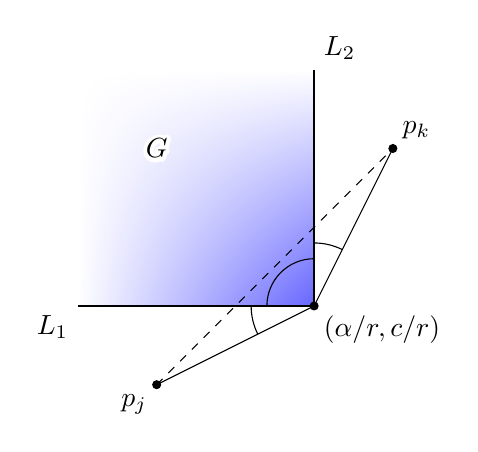
\begin{tikzpicture}
\contourlength{0.5mm};
\coordinate[label=below left:$L_1$] (L1) at (0,0);
\coordinate[label=above right:$L_2$] (L2) at (3,3);
\coordinate[label=below right:{$(\alpha/r,c/r)$}] (g) at (3,0);
\coordinate[label=below left:$p_j$] (pj) at (1,-1);
\coordinate[label=above right:$p_k$] (pk) at (4,2);

\shade[lower right=blue!60!white] (L1) rectangle (3,3);
\draw[thick] (g)--(L1);
\draw[thick] (g)--(L2);
\node at (1,2) {\contour{white}{$G$}};
\filldraw (g) circle(0.05);
\filldraw (pj) circle(0.05);
\filldraw (pk) circle(0.05);
\draw (g)--(pj);
\draw (g)--(pk);
\draw[dashed] (pj)--(pk);

\begin{scope}
\path[clip] (g) -- (pj) -- (L1);
\draw (g) circle (0.8);
\end{scope}
%\node[scale=0.5] at (2.3,-0.1)  {$\sphericalangle p_j L_1$};

\begin{scope}
\path[clip] (g) -- (L1) -- (L2);
\draw (g) circle (0.6);
\end{scope}
%\node[scale=0.5] at (2.6,0.2) {$\sphericalangle L_1 L_2$};

\begin{scope}
\path[clip] (g) -- (L2) -- (pk);
\draw (g) circle (0.8);
\end{scope}
%\node[scale=0.5] at (3.2,0.9) {$\sphericalangle L_2 p_k$};
\end{tikzpicture}
\end{wrapfigure}

Step one and two of the algorithm are straightforward, but how do we find $j,k$ with $\overline{p_j p_k}\cap G\neq \emptyset$? We have seen that the area $G$ is the intersection of two half-planes, lets call them $L_1$ and $L_2$. The line $\overline{p_j p_k}$ crosses $G$ if and only if
\begin{equation*}
\sphericalangle p_j L_1+\sphericalangle L_1 L_2+\sphericalangle L_2 p_k\leq \pi
\end{equation*}
	
The angle $\sphericalangle L_1 L_2$ is independent from $j$ and $k$, which means that we can minimize $\sphericalangle p_j L_1$ and $\sphericalangle L_2 p_k$   seperately.

}


\vspace{1cm}

%TODO algo sources
Where is the quantum speed-up? In step two of the algorithm we have to check if one of the $p_i$'s is in $G$. If we implement the function $i\to$"Is $p_i\in G$?" as a  quantum circuit, then Grover search can be used to find such a $p_i$ in $\mathcal{O}(\sqrt{m})$. Similarily we have to minimize the angles $\sphericalangle p_j L_1$ and $\sphericalangle L_2 p_k$ for step 3, so if we implement the functions $i\to\sphericalangle p_i L_1$ and $i\to \sphericalangle L_2 p_k$ as quantum circuits, then the quantum minimum-finding algorithm of Dürr and Høyer can be used to minimize them in $\mathcal{O}(\sqrt{m})$.


%Chapter 4?
\subsection{Runtime of the SDP solver}

TODO: The calculation of the runtime is not that complicated, but we would have to use a few formulas we didnt explain or use before. Basically its (number of iterations) * (cost of oracle + times the oracle uses $\Tr(A_j)$ * time for its calculation). 

SDP:
\begin{equation*}
\tilde{\mathcal{O}}\left(\sqrt{mn}s^2\left(\frac{Rr}{\varepsilon}\right)^8\right)
\end{equation*}

LP:
\begin{equation*}
\tilde{\mathcal{O}}\left(\sqrt{mn}s^2\left(\frac{Rr}{\varepsilon}\right)^5\right)
\end{equation*}

Classicaly:
\begin{equation*}
\tilde{\mathcal{O}}\left(mns\left(\frac{Rr}{\varepsilon}\right)^4+ns\left(\frac{Rr}{\varepsilon}\right)^7\right)
\end{equation*}

\subsection{Downsides}
TODO: Still have to decide with Markus which ones we include, and who does what. Something will be in the final version of this document. The ideas are: 2-sparse dual solutions $\rightarrow$ high amount of iterations if all optimal solutions are dense. If we could find an oracle with lower width, then it couldnt be used for all SDPs. High exponent around $Rr/\varepsilon$, we dont know useful examples where this is small.

\subsection{Conclusions}
TODO

\vspace{1cm}
TODO: Sources

% bibliography
\printbibliography

\end{document}